% Source: outputs/illustrations/gastroscopy_sequence_warm_final_no_labels/
%         case_0173_gaussian_clusters.pdf (copied without changing the artwork).
% The accompanying selection.json marks the coordinates as schematic_only;
% they are not measured endoscopic spatial coordinates or ACPE outputs.
% Shared caption: English in main.tex; English and Chinese in draft.tex.
\begin{figure}[t]
    \centering
    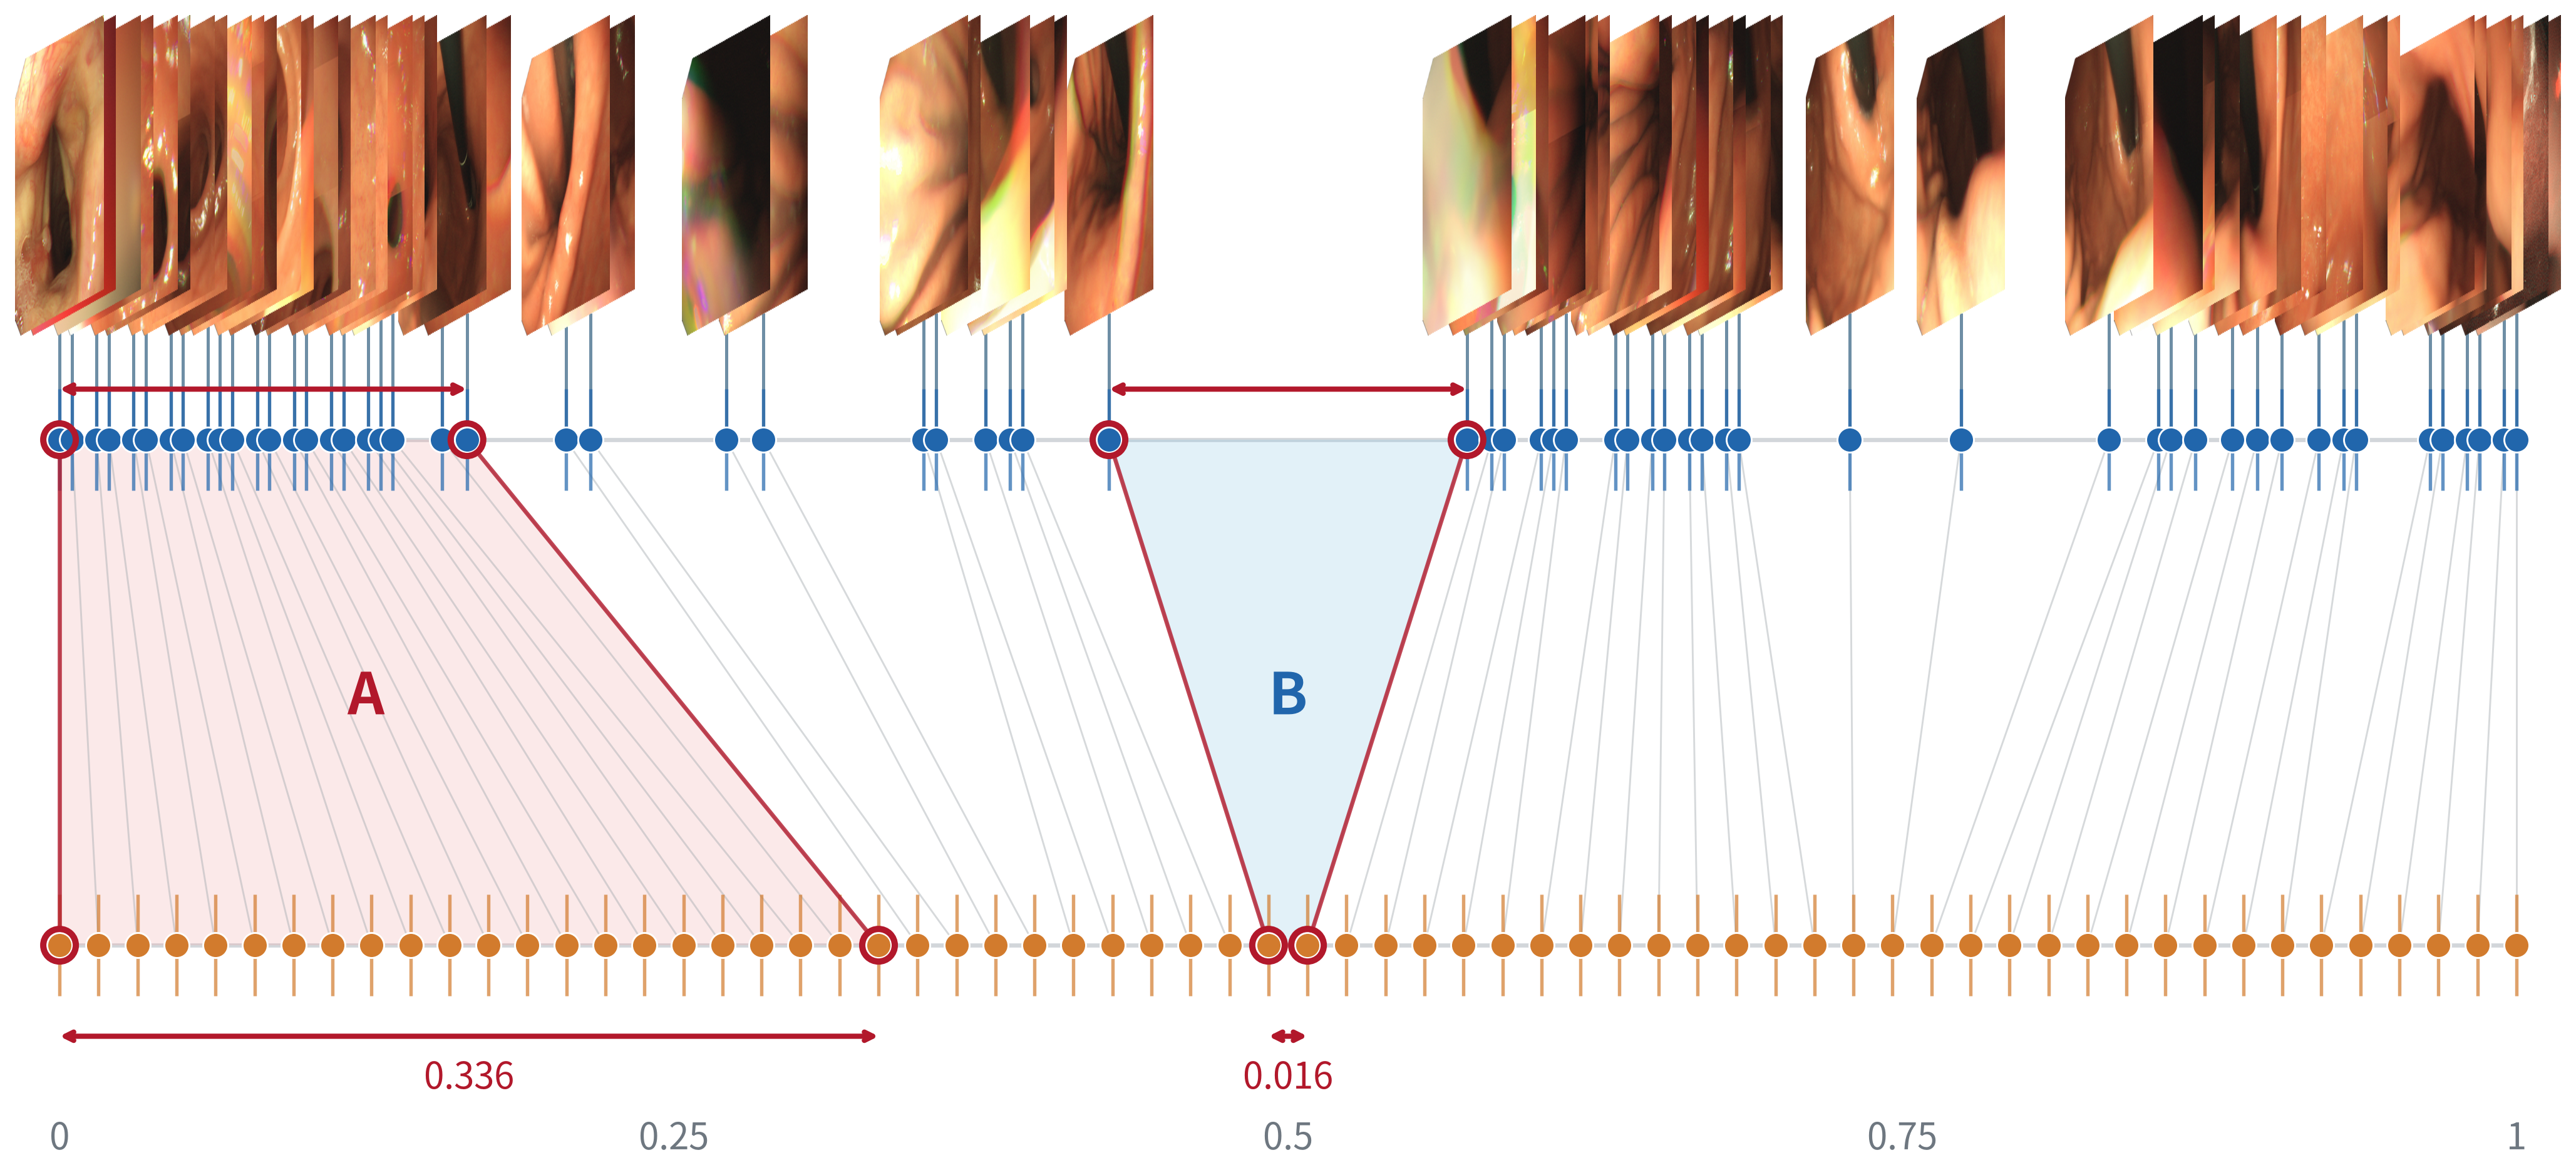
\includegraphics[width=\linewidth]{fig/figure1.pdf}
    \caption[Positional-reference mismatch in discrete examination images.]{%
        Illustration of positional-reference mismatch in discrete examination images.
        Blue and orange nodes show schematic spatial positions and uniformly spaced positional encoding (PE) coordinates, respectively; gray lines connect corresponding images.
        Equal index spacing expands a densely sampled spatial interval (A) and compresses a large gap between consecutive samples (B), distorting inter-image positional relationships.
        Numerical annotations denote normalized PE intervals.
        \cntranslation{%
            离散检查图像的位置参照错配示意图。蓝色与橙色节点分别表示示意性空间位置和等距位置编码（PE）坐标，灰色连线连接对应图像。等距索引将密集采样区间的空间跨度拉大（A），并将相邻采样图像间较大的空间间隔压缩（B），从而扭曲图像间的位置关系。数值标注表示归一化的 PE 间距。
        }%
    }
    \label{fig:position_mismatch}
\end{figure}
